\documentclass[twoside]{book}

% Packages required by doxygen
\usepackage{fixltx2e}
\usepackage{calc}
\usepackage{doxygen}
\usepackage[export]{adjustbox} % also loads graphicx
\usepackage{graphicx}
\usepackage[utf8]{inputenc}
\usepackage{makeidx}
\usepackage{multicol}
\usepackage{multirow}
\PassOptionsToPackage{warn}{textcomp}
\usepackage{textcomp}
\usepackage[nointegrals]{wasysym}
\usepackage[table]{xcolor}

% NLS support packages
\usepackage[brazil]{babel}
% Font selection
\usepackage[T1]{fontenc}
\usepackage[scaled=.90]{helvet}
\usepackage{courier}
\usepackage{amssymb}
\usepackage{sectsty}
\renewcommand{\familydefault}{\sfdefault}
\allsectionsfont{%
  \fontseries{bc}\selectfont%
  \color{darkgray}%
}
\renewcommand{\DoxyLabelFont}{%
  \fontseries{bc}\selectfont%
  \color{darkgray}%
}
\newcommand{\+}{\discretionary{\mbox{\scriptsize$\hookleftarrow$}}{}{}}

% Page & text layout
\usepackage{geometry}
\geometry{%
  a4paper,%
  top=2.5cm,%
  bottom=2.5cm,%
  left=2.5cm,%
  right=2.5cm%
}
\tolerance=750
\hfuzz=15pt
\hbadness=750
\setlength{\emergencystretch}{15pt}
\setlength{\parindent}{0cm}
\setlength{\parskip}{3ex plus 2ex minus 2ex}
\makeatletter
\renewcommand{\paragraph}{%
  \@startsection{paragraph}{4}{0ex}{-1.0ex}{1.0ex}{%
    \normalfont\normalsize\bfseries\SS@parafont%
  }%
}
\renewcommand{\subparagraph}{%
  \@startsection{subparagraph}{5}{0ex}{-1.0ex}{1.0ex}{%
    \normalfont\normalsize\bfseries\SS@subparafont%
  }%
}
\makeatother

% Headers & footers
\usepackage{fancyhdr}
\pagestyle{fancyplain}
\fancyhead[LE]{\fancyplain{}{\bfseries\thepage}}
\fancyhead[CE]{\fancyplain{}{}}
\fancyhead[RE]{\fancyplain{}{\bfseries\leftmark}}
\fancyhead[LO]{\fancyplain{}{\bfseries\rightmark}}
\fancyhead[CO]{\fancyplain{}{}}
\fancyhead[RO]{\fancyplain{}{\bfseries\thepage}}
\fancyfoot[LE]{\fancyplain{}{}}
\fancyfoot[CE]{\fancyplain{}{}}
\fancyfoot[RE]{\fancyplain{}{\bfseries\scriptsize Gerado por Doxygen }}
\fancyfoot[LO]{\fancyplain{}{\bfseries\scriptsize Gerado por Doxygen }}
\fancyfoot[CO]{\fancyplain{}{}}
\fancyfoot[RO]{\fancyplain{}{}}
\renewcommand{\footrulewidth}{0.4pt}
\renewcommand{\chaptermark}[1]{%
  \markboth{#1}{}%
}
\renewcommand{\sectionmark}[1]{%
  \markright{\thesection\ #1}%
}

% Indices & bibliography
\usepackage{natbib}
\usepackage[titles]{tocloft}
\setcounter{tocdepth}{3}
\setcounter{secnumdepth}{5}
\makeindex

% Hyperlinks (required, but should be loaded last)
\usepackage{ifpdf}
\ifpdf
  \usepackage[pdftex,pagebackref=true]{hyperref}
\else
  \usepackage[ps2pdf,pagebackref=true]{hyperref}
\fi
\hypersetup{%
  colorlinks=true,%
  linkcolor=blue,%
  citecolor=blue,%
  unicode%
}

% Custom commands
\newcommand{\clearemptydoublepage}{%
  \newpage{\pagestyle{empty}\cleardoublepage}%
}

\usepackage{caption}
\captionsetup{labelsep=space,justification=centering,font={bf},singlelinecheck=off,skip=4pt,position=top}

%===== C O N T E N T S =====

\begin{document}

% Titlepage & ToC
\hypersetup{pageanchor=false,
             bookmarksnumbered=true,
             pdfencoding=unicode
            }
\pagenumbering{roman}
\begin{titlepage}
\vspace*{7cm}
\begin{center}%
{\Large Tratamento de polígonos }\\
\vspace*{1cm}
{\large Gerado por Doxygen 1.8.11}\\
\end{center}
\end{titlepage}
\clearemptydoublepage
\tableofcontents
\clearemptydoublepage
\pagenumbering{arabic}
\hypersetup{pageanchor=true}

%--- Begin generated contents ---
\chapter{poligonos\+Qt}
\label{md_README}
\hypertarget{md_README}{}
\input{md_README}
\chapter{Índice Hierárquico}
\section{Hierarquia de Classes}
Esta lista de hierarquias está parcialmente ordenada (ordem alfabética)\+:\begin{DoxyCompactList}
\item \contentsline{section}{Point}{\pageref{class_point}}{}
\item \contentsline{section}{Poligono}{\pageref{class_poligono}}{}
\begin{DoxyCompactList}
\item \contentsline{section}{Retangulo}{\pageref{class_retangulo}}{}
\end{DoxyCompactList}
\end{DoxyCompactList}

\chapter{Índice dos Componentes}
\section{Lista de Componentes}
Aqui estão as classes, estruturas, uniões e interfaces e suas respectivas descrições\+:\begin{DoxyCompactList}
\item\contentsline{section}{\hyperlink{class_point}{Point} }{\pageref{class_point}}{}
\item\contentsline{section}{\hyperlink{class_poligono}{Poligono} }{\pageref{class_poligono}}{}
\item\contentsline{section}{\hyperlink{class_retangulo}{Retangulo} }{\pageref{class_retangulo}}{}
\end{DoxyCompactList}

\chapter{Classes}
\hypertarget{class_point}{}\section{Referência da Classe Point}
\label{class_point}\index{Point@{Point}}


{\ttfamily \#include $<$point.\+h$>$}

\subsection*{Métodos Públicos}
\begin{DoxyCompactItemize}
\item 
\hyperlink{class_point_a06c32166c2ad9eac25799ef189b49683}{Point} (float \+\_\+x=0, float \+\_\+y=0)\hypertarget{class_point_a06c32166c2ad9eac25799ef189b49683}{}\label{class_point_a06c32166c2ad9eac25799ef189b49683}

\begin{DoxyCompactList}\small\item\em Inicializa o ponto com as coordenadas $x$ e $y$ informadas, caso não seja informado as coordenadas do ponto elas inicializaram com zero. \end{DoxyCompactList}\item 
void \hyperlink{class_point_a428a1676e2fdec6753c42011a1d59d18}{setX} (float \+\_\+x)\hypertarget{class_point_a428a1676e2fdec6753c42011a1d59d18}{}\label{class_point_a428a1676e2fdec6753c42011a1d59d18}

\begin{DoxyCompactList}\small\item\em Definir o valor da coordenada $x$ do ponto. \end{DoxyCompactList}\item 
void \hyperlink{class_point_a9868c4601b0ea0c2d0de20fe41ee0e49}{setY} (float \+\_\+y)\hypertarget{class_point_a9868c4601b0ea0c2d0de20fe41ee0e49}{}\label{class_point_a9868c4601b0ea0c2d0de20fe41ee0e49}

\begin{DoxyCompactList}\small\item\em Definir o valor da coordenada $y$ do ponto. \end{DoxyCompactList}\item 
void \hyperlink{class_point_ab5385c6d9bfa841e641e4709fc9f14cc}{set\+XY} (float \+\_\+x, float \+\_\+y)\hypertarget{class_point_ab5385c6d9bfa841e641e4709fc9f14cc}{}\label{class_point_ab5385c6d9bfa841e641e4709fc9f14cc}

\begin{DoxyCompactList}\small\item\em Definindo o valores das coordenadas $x$ e $y$ do ponto. \end{DoxyCompactList}\item 
float \hyperlink{class_point_acc27466778cc87a662bba40268c4c0c8}{getX} ()\hypertarget{class_point_acc27466778cc87a662bba40268c4c0c8}{}\label{class_point_acc27466778cc87a662bba40268c4c0c8}

\begin{DoxyCompactList}\small\item\em Retorna o valor da coordenada $x$. \end{DoxyCompactList}\item 
float \hyperlink{class_point_a3cccbca94719ddde353cce86ce0e2f64}{getY} ()\hypertarget{class_point_a3cccbca94719ddde353cce86ce0e2f64}{}\label{class_point_a3cccbca94719ddde353cce86ce0e2f64}

\begin{DoxyCompactList}\small\item\em Retorna o valor da coordenada $y$. \end{DoxyCompactList}\item 
\hyperlink{class_point}{Point} \hyperlink{class_point_a9dbea84b07b0a8ec3bbb9e58b3d15899}{add} (\hyperlink{class_point}{Point} p1)\hypertarget{class_point_a9dbea84b07b0a8ec3bbb9e58b3d15899}{}\label{class_point_a9dbea84b07b0a8ec3bbb9e58b3d15899}

\begin{DoxyCompactList}\small\item\em Adiciona as coordenadas $(x,y)$ do ponto com as coordenadas de um ponto $P1(x_1,y_1)$ fornecido, armazenando o resultado $(x+x_1,y+y_1)$ nas coordenadas de um novo ponto, que deverá ser retornado para o cliente da classe. \end{DoxyCompactList}\item 
\hyperlink{class_point}{Point} \hyperlink{class_point_a9cf2c53b0a4e6282a6712824bb4e9b00}{sub} (\hyperlink{class_point}{Point} p1)\hypertarget{class_point_a9cf2c53b0a4e6282a6712824bb4e9b00}{}\label{class_point_a9cf2c53b0a4e6282a6712824bb4e9b00}

\begin{DoxyCompactList}\small\item\em Subtrai as coordenadas $(x,y)$ do ponto com as coordenadas de um ponto $P1(x_1,y_1)$ fornecido, armazenando o resultado $(x−x_1,y−y_1)$ nas coordenadas de um novo ponto, que deverá ser retornado para o cliente da classe. \end{DoxyCompactList}\item 
float \hyperlink{class_point_abd2618d1f505d9392893273a66e7c9b2}{norma} ()\hypertarget{class_point_abd2618d1f505d9392893273a66e7c9b2}{}\label{class_point_abd2618d1f505d9392893273a66e7c9b2}

\begin{DoxyCompactList}\small\item\em Retorna o cálculo da distância do ponto para a origem do sistema de coordenadas. \end{DoxyCompactList}\item 
void \hyperlink{class_point_aaa6b1904e9e73484651bb5b1191e0f18}{translada} (float \+\_\+a, float \+\_\+b)\hypertarget{class_point_aaa6b1904e9e73484651bb5b1191e0f18}{}\label{class_point_aaa6b1904e9e73484651bb5b1191e0f18}

\begin{DoxyCompactList}\small\item\em Translada o ponto $(x,y)$ de $(+a,+b)$, de modo que, após a execução do método, as coordenadas do ponto serão $(x+a,y+b)$. \end{DoxyCompactList}\item 
void \hyperlink{class_point_a1fb5c2501c27ab2cbc99d06c2a26a741}{imprime} ()\hypertarget{class_point_a1fb5c2501c27ab2cbc99d06c2a26a741}{}\label{class_point_a1fb5c2501c27ab2cbc99d06c2a26a741}

\begin{DoxyCompactList}\small\item\em Imprime o ponto na forma $(x,y)$. \end{DoxyCompactList}\end{DoxyCompactItemize}


\subsection{Descrição Detalhada}
A classe point foi criada para realizar o tratamento de pontos. 

A documentação para esta classe foi gerada a partir dos seguintes arquivos\+:\begin{DoxyCompactItemize}
\item 
point.\+h\item 
point.\+cpp\end{DoxyCompactItemize}

\hypertarget{class_poligono}{}\section{Referência da Classe Poligono}
\label{class_poligono}\index{Poligono@{Poligono}}


{\ttfamily \#include $<$poligono.\+h$>$}



Diagrama de Hierarquia para Poligono\+:\nopagebreak
\begin{figure}[H]
\begin{center}
\leavevmode
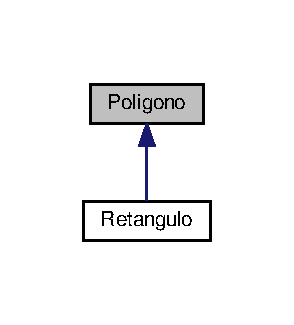
\includegraphics[width=141pt]{class_poligono__inherit__graph}
\end{center}
\end{figure}
\subsection*{Métodos Públicos}
\begin{DoxyCompactItemize}
\item 
\hyperlink{class_poligono_a9311a9a1496878c09c8508b3636e2870}{Poligono} ()\hypertarget{class_poligono_a9311a9a1496878c09c8508b3636e2870}{}\label{class_poligono_a9311a9a1496878c09c8508b3636e2870}

\begin{DoxyCompactList}\small\item\em Inicializa o número de vertices com zero. \end{DoxyCompactList}\item 
void \hyperlink{class_poligono_a0784e2fb0149f6923a42bfabfb073719}{set\+Vertice} (float \+\_\+x, float \+\_\+y)\hypertarget{class_poligono_a0784e2fb0149f6923a42bfabfb073719}{}\label{class_poligono_a0784e2fb0149f6923a42bfabfb073719}

\begin{DoxyCompactList}\small\item\em Definir um vertice do polígono. Assumindo que os vértices deverão ser inseridos conforme a sequência (anti-\/horária) em que figuram ao redor do polígono. As arestas do polígono serão então compostas pelos segmentos $(x_0,y_0)→(x_1,y_1)$, $(x_1,y_1)→(x_2,y_2)$ etc., com exceção da última aresta, que será formada pelo segmento $(x_{N−1},y_{N−1})→(x_0,y_0)..$. \end{DoxyCompactList}\item 
float \hyperlink{class_poligono_a1ae7255db591e28a3a35293210033811}{get\+Cont\+Vertices} ()\hypertarget{class_poligono_a1ae7255db591e28a3a35293210033811}{}\label{class_poligono_a1ae7255db591e28a3a35293210033811}

\begin{DoxyCompactList}\small\item\em Retorna o número de vertices inseridos. \end{DoxyCompactList}\item 
float \hyperlink{class_poligono_a7f66c446f86c19118663ef1b2c8a4be6}{area} ()\hypertarget{class_poligono_a7f66c446f86c19118663ef1b2c8a4be6}{}\label{class_poligono_a7f66c446f86c19118663ef1b2c8a4be6}

\begin{DoxyCompactList}\small\item\em Retorna o cálculo da área do polígono armazenado. \end{DoxyCompactList}\item 
void \hyperlink{class_poligono_aafacd43b0918e0765fbb42d9aad5bb35}{translada} (float \+\_\+a, float \+\_\+b)\hypertarget{class_poligono_aafacd43b0918e0765fbb42d9aad5bb35}{}\label{class_poligono_aafacd43b0918e0765fbb42d9aad5bb35}

\begin{DoxyCompactList}\small\item\em Translada o polígono armazenado. \end{DoxyCompactList}\item 
void \hyperlink{class_poligono_adaee71aa07241ba4e7f751a01163738a}{rotacionar} (float angulo)\hypertarget{class_poligono_adaee71aa07241ba4e7f751a01163738a}{}\label{class_poligono_adaee71aa07241ba4e7f751a01163738a}

\begin{DoxyCompactList}\small\item\em Rotaciona o polígono armazenado. \end{DoxyCompactList}\item 
void \hyperlink{class_poligono_ac22d76a087d08ea82627be416404ae15}{print} ()\hypertarget{class_poligono_ac22d76a087d08ea82627be416404ae15}{}\label{class_poligono_ac22d76a087d08ea82627be416404ae15}

\begin{DoxyCompactList}\small\item\em Imprimir a estrutura do polígino armazenado na forma $(x_0,y_0)→(x_1,y_1)→(x_2,y_2)→…$. \end{DoxyCompactList}\end{DoxyCompactItemize}


\subsection{Descrição Detalhada}
A classe Polígono foi criada para realizar o tratamento de polígonos. 

A documentação para esta classe foi gerada a partir dos seguintes arquivos\+:\begin{DoxyCompactItemize}
\item 
poligono.\+h\item 
poligono.\+cpp\end{DoxyCompactItemize}

\hypertarget{class_retangulo}{}\section{Referência da Classe Retangulo}
\label{class_retangulo}\index{Retangulo@{Retangulo}}


{\ttfamily \#include $<$retangulo.\+h$>$}



Diagrama de Hierarquia para Retangulo\+:\nopagebreak
\begin{figure}[H]
\begin{center}
\leavevmode
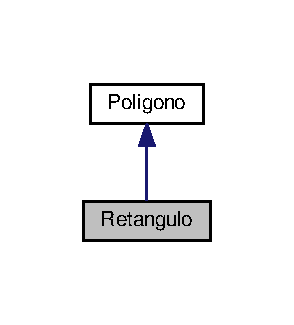
\includegraphics[width=141pt]{class_retangulo__inherit__graph}
\end{center}
\end{figure}


Diagrama de colaboração para Retangulo\+:\nopagebreak
\begin{figure}[H]
\begin{center}
\leavevmode
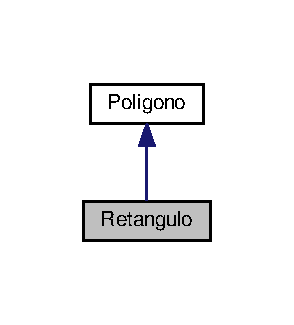
\includegraphics[width=141pt]{class_retangulo__coll__graph}
\end{center}
\end{figure}
\subsection*{Métodos Públicos}
\begin{DoxyCompactItemize}
\item 
\hyperlink{class_retangulo_a53fcd5f31b65aae653972f2d0db004e4}{Retangulo} (float \+\_\+x=0, float \+\_\+y=0, float \+\_\+largura=0, float \+\_\+altura=0)\hypertarget{class_retangulo_a53fcd5f31b65aae653972f2d0db004e4}{}\label{class_retangulo_a53fcd5f31b65aae653972f2d0db004e4}

\begin{DoxyCompactList}\small\item\em Inicializa a posição $(x,y)$ e dimensões largura e altura do retangulo, caso os dados não forem informados assumiram o valor zero. \end{DoxyCompactList}\end{DoxyCompactItemize}


\subsection{Descrição Detalhada}
A classe \hyperlink{class_retangulo}{Retangulo} foi criada para realizar o tratamento de retangulos. 

A documentação para esta classe foi gerada a partir dos seguintes arquivos\+:\begin{DoxyCompactItemize}
\item 
retangulo.\+h\item 
retangulo.\+cpp\end{DoxyCompactItemize}

%--- End generated contents ---

% Index
\backmatter
\newpage
\phantomsection
\clearemptydoublepage
\addcontentsline{toc}{chapter}{Índice}
\printindex

\end{document}
